\documentclass[a4paper]{article}

%% Language and font encodings
\usepackage[english]{babel}
\usepackage[T1]{fontenc}

%% Sets page size and margins
\usepackage[a4paper,top=3cm,bottom=2cm,left=3cm,right=3cm,marginparwidth=1.75cm]{geometry}

%% Useful packages
\usepackage{amsmath}
\usepackage{graphicx}
\usepackage[colorinlistoftodos]{todonotes}
\usepackage[colorlinks=true, allcolors=blue]{hyperref}

\title{Week 3 Journal}
\author{Kevin Cardenas}

\begin{document}
\maketitle

\section{In Class Browsing and Scanning Exercise}

We were asked to browse the following three papers:
\begin{enumerate}
    \item \url{http://www.mecs-press.org/ijcnis/ijcnis-v10-n5/IJCNIS-V10-N5-7.pdf}
    \item \url{https://ieeexplore.ieee.org/iel5/5361789/5362099/05362133.pdf?casa_token=GkRt8Bd-LaIAAAAA:-otKOXZwhusHHiieU9ODZBQI4EEQj6fEqPcA_oOTLxGiHQdQLGfVxsnIHGUYi-OWpgz_L0HDL_V86A}
    \item \url{https://journals.plos.org/plosone/article?id=10.1371/journal.pone.0155781}
\end{enumerate}

After scanning the three articles, I found the third one most interesting and most credible. The first paper did not make many connections to related work and had large amounts of code written in the article. The second paper's abstract seemed short, vague and a little non-technical. I chose to scan the third paper because I came up with most of the C's within the first minute of browsing. The web page made it extremely easy to find key information and the author's did an excellent job presenting the highlights in their abstract and introduction.  

\section{Browsing}

\subsection{Journal Choice}
I chose to browse articles in the Computers in Human Behavior journal because it has an h-index of 203 and has issues dating back to 1985. I hope to learn more about Human Computer Interaction (HCI), specifically focusing on the psychology of humans interacting with computers. 

\begin{figure}[!htb]
\centering
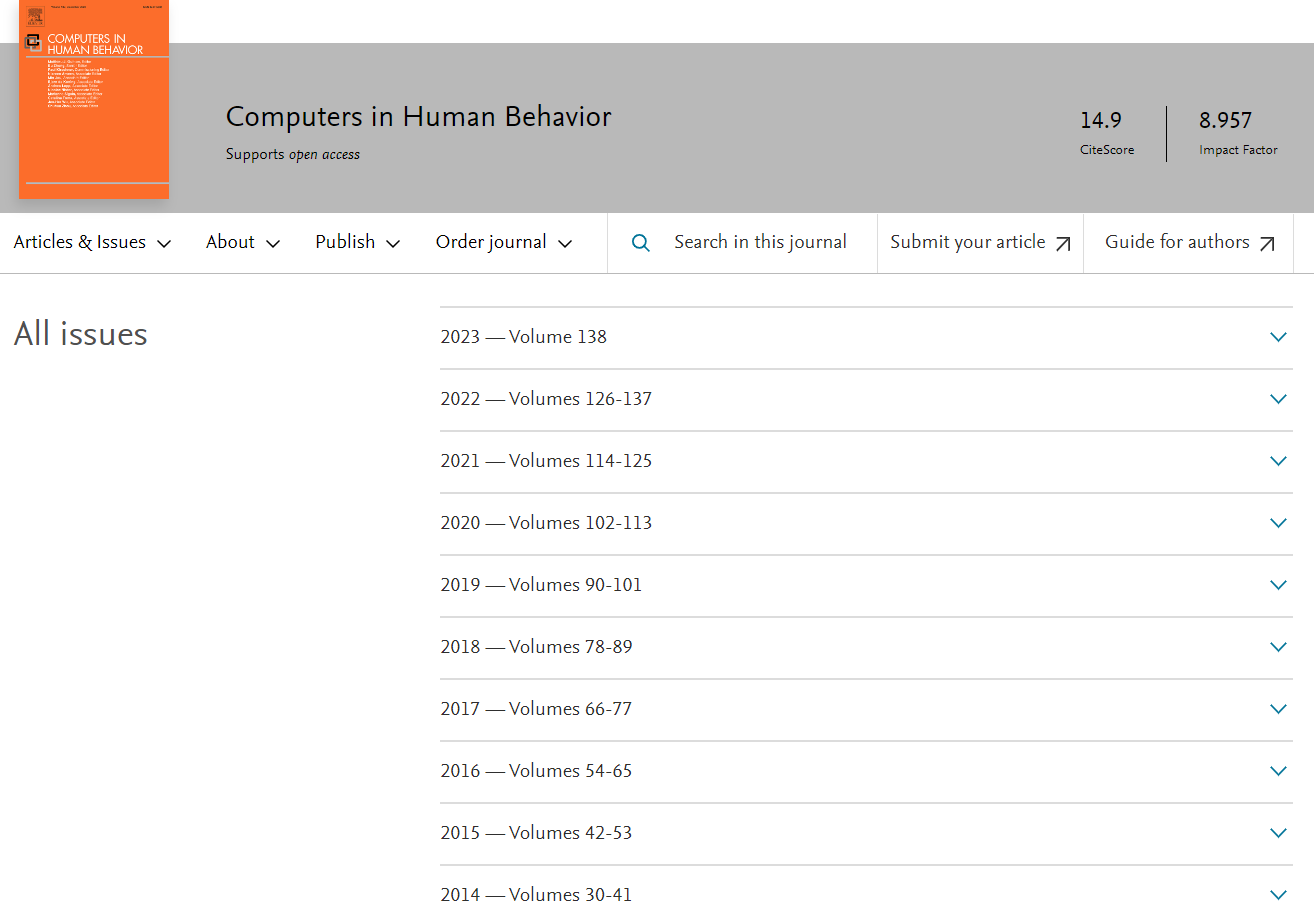
\includegraphics[width=0.7\textwidth]{figures/j02.PNG}
\caption{\label{fig:search} Computers in Human Behavior \cite{noauthor_editorial_2022}}
\end{figure}

\subsection{Browse 50 Papers}
I went through 50 papers in this journal starting with the latest issue (Volume 138) that is open until January of 2023. I would add the paper to Zotero using the Chorme plugin, start a stopwatch, read the abstract/figures/captions, priority score the paper from 1-5 (best to worst), and stop the timer. I then added the time and brief note summarizing why I chose to move the paper to my scan list or discard it.


\section{Scanning}
\begin{enumerate}
    \item This paper explores the possibility of utilizing virtual humans to share emotional distress with compared to the traditional methods of talking to friends or a professional therapist. There are numerous citations in the opening paragraphs for social sharing, means for people seeking help, virtual humans in health care, and more. The results indicate that people feel better after talking to a virtual human and provide cognitive and emotional support. \cite{pauw_avatar_2022}
    
    \item The paper provides the results of an experiment run to extract significant features of Instagram users and their evaluation of people's body appearance in pictures. They used body shape and body part (face-only, body-only) from 165 images along with participants' eye movements to show the effects of these images on viewers. The authors provide good context for their work and appear credible with multiple citations in each aspect of their research (social comparison, body dissatisfaction, and eye-tracking). \cite{scott_thinstagram_2023}
    
    \item This paper expands upon research done on the General Learning Model applied to post-video game attentional bias toward prosocial information and behaviors. It provides some credibility from previous work, but is ventures into a new direction. This article has a fairly high cost because I would have to learn more about prosocial behaviors and how to measure them. \cite{yin_effects_2022}
    
    \item This paper explores the gendering of machine agents which seems to be a fairly new field of study because the author did not mention any previous work. The research does not seem the most credible for that reason and because they only have around 650 observations for their survey. This seems like a fairly large number, but when dealing with qualitative data (like a survey) more data is required. It doesn't appear the author is providing much or any contributions, rather an interesting look at how people view machine agents. \cite{fortunati_is_2022}
    
    \item This paper aims to answer how emotionally charged stories can be used to engage audiences on social media. Similar to the previous paper, this paper does not provide any link to previous research and has a smaller number of observations ($N = 403$). \cite{zhao_primacy_2022}
    
    \item This paper provides insight to ways ePortfolio implementation can aid teaching and learning. The author makes several citations to previous work especially to help define new terminology. The analysis piece of this article appears to be less technical which hinders their credibility in my opinion. \cite{pospisilova_reforming_2023}
    
    \item This paper examines computer-mediated communications (CMC) and summarizes three types of online behavior. This paper immediately loses credibility when looking at the conclusion. The authors continue to provide theoretical background for their work and do not summarize the key findings of their work. The paper seemingly speculates the taxonomy of CMC without much support from any analytical study. \cite{kaye_the_2022}
    
    \item This paper provides non-technical insight about how to integrate AI into education from a teacher's pedagogical perspective. The initial allure of utilizing AI for teaching is lost when the author focuses on the teacher's knowledge of using AI-based tools in education. The paper focuses primarily on the pedagogy behind using AI-tools in the classroom and not the tools themselves or their effectiveness. \cite{celik_towards_2023}
\end{enumerate}

\section{Critically \& Creatively Read}
\begin{enumerate}
    \item The avatar will see you now: Support from a virtual human provides socio-emotional benefits \cite{pauw_avatar_2022}
    
    Notes: 115 participants. 2 cameras for facial expressions and interaction with virtual human. 2 personal issues (anger, worry). Intro conversation with Julie and then recall, followed by survey questions. Then another recall without an intro conversation followed by survey. Used 7-point Likert scale. Assume people know how to quantify their emotions. Gender/ethnicity and control questions balanced. Used ANOVA. Participants experienced somewhat higher emotional intensity when discussing the worry-evoking event as compared to the anger-evoking event. The observed increase in affect was equally strong across emotional and cognitive support provision. emotional support and cognitive support were associated with similar affect across both anger and worry-evoking events. Making claims when ANOVA results were not statistically significant ("indicating that the provision of emotional and cognitive support was judged to be similarly effective"). Lack of control group, comparing one people who share. What is perceived support efficacy based on? All of the virtual human questions/responses were pre-recorded. Findings indicate that talking to a virtual human effectively reduces the emotional intensity of the shared emotional experience. This could apply to teaching empathy using AI-driven VR experiences because it shows the possibility of connection/learning/healing with a virtual human. Could use similar experiment construct/approach with different factors/levels to measure learning instead of emotional healing.
    
    \item “Thinstagram”: Image content and observer body satisfaction influence the when and where of eye movements during instagram image viewing \cite{scott_thinstagram_2023}
    
    Notes: Problem - Social comparison and body dissatisfaction. How are the pictures consumed by female users. Recorded eye movements of users looking at face images and body images with a representative proportion of under, average and over weight people. Background of Instagram use and social comparison/body dissatisfaction, eye-tracking (gaze patterns, areas of interest, fixation frequency, etc). Prev studies found healthy women look at good parts of themselves and "ugly" parts of other. Opposite for people who have eating disorders and are unhealthy. 3x4 pictures of various weight and body area focus (face vs body). Seek to compare which type of image most attracted to with own self image. Features are first pass time, total fixation duration (dwell time), fixation count and visit count. Does not include order in which area of interests are visited. Body > face // under weight > over weight // lower head satisfaction less underweight face. Used 7-point Likert scale to evaluate weight of pictures. Separated these evaluators from final study. Used ANOVA (3 x 2: Body Shape x Part). "We performed regression analyses globally, taking forward candidate predictors based on prior general linear model and correlational analyses." WITHOUT CITATION... What type of regression was used? Is p<0.1 good for this field of study? Why compare to p<0.05? Terrible $R^2$ results not explained. Small $n$ probably doesn't help. This doesn't seem to make a meaningful contribution, but confirms previous studies. Using these eye-tracking metrics could be interesting to add to research of learning empathy with AI-driven VR. Fitting a model might be extremely challenging with low amount of data points. 
\end{enumerate}

\section{Lessons Learned}
I learned a lot from this week's journal! Unfortunately, one of the most important things I learned was that I have \textbf{a lot} of learning and work to do to get better at finding journals and browsing/scanning articles. Everything about this exercise took more time than I expected: Finding a journal that seemed like it aligned with my research area, browsing took around two minutes for a large majority of the papers I found, and scanning also took more time than expected.

A second important lesson I learned is to choose a journal that grants free access to all of the papers. \href{https://www.sciencedirect.com/}{Science Direct} published by Elsevier does not have very many papers fully available. Of the 50 papers I browsed, there were only 9 papers that included the full PDF.

After browsing through about 10-15 papers, I started to realize that I don't think Computers in Human Behavior is quite the journal for my research area. When I think of the term "Human Behavior", I think of personal/individual behavior. However, this journal focuses on social behavior with a heavy presence of research about the impacts of social media. Most of the journals had a very light sprinkle of statistics and possibly some logistic regression, but didn't seem very technically rigorous or credible.

I am learning more about setting up the .bib file, but still am unsure of a "proper" style for author names, capitalization of titles, URLs, etc. I am also unsure how to include the annotations after a decent web search. 

I am planning on completing this exercise again, but with another journal to practice these skills. Also, I think it would be beneficial to hopefully find a journal that hosts research that is more interesting/applicable to my research area. I would love the opportunity to sit down with Dr. Boult and talk him through how I approached finding a journal and ask for recommendations on how to browse and scan more efficiently.

\newpage
\bibliographystyle{IEEEtran}
\bibliography{j02}
\nocite{*}

\end{document}